\chapter{Image and Graphics}
An image is a spatial representation of an object, a two-dimensional or three-dimensional scene or another image. It can be real or virtual. An image may be abstractly thought of as a continuous function defining usually rectangular region of a plane.

A recorded image may be in a photographic, analog video signal or digital format. In computer vision, an image is usually a recorded image such as a-video-image, digital image or picture. In computer graphics, an image is always a digital image. In multimedia applications, all formats can be presented.

Graphics are normally created in a graphics application and internally represented as an assemblage of objects such as lines, curves, or circles. Attributes such as style, width, and color define the appearance of graphics. We say that the representation is aware of the semantic contents. The objects graphics are composed of can be individually deleted, added, moved, or modified later.⎄ In contrast, images can be from the real world or virtual and are not editable in the sense given above. They ignore the semantic contents. They are described as spatial arrays of values. 

The smallest addressable image element is called a \textit{pixel}. The array, and thus the set of pixels, is called a \textit{bitmap}. 

\subsubsection*{Drawback of Bitmaps}
The drawback of bitmaps is that they need much more storage capacity than graphics.

\subsubsection*{Advantage of Bitmaps}
Their advantage is that no processing is necessary before displaying them, unlike graphics where the abstract definition must be processed first to produce a bitmap.

\section{Basic Concepts, Digital Image Processing and Format and Graphics Format}

\subsection{Basic Concepts}
An image might be thought of as a function with resulting values of the light intensity at each point over a planar region. For digital computer operations, this function needs to be sampled at discrete intervals. The sampling quantizes the intensity values into discrete levels.

\subsection*{Digital Image Representation}
A digital image is represented by a matrix of numeric values each representing a quantized intensity value. When $ I $ is a two-dimensional matrix, then $ I(r, c) $ is the intensity value at the position corresponding to row $ r $ and column $ c $ of the matrix.

\begin{itemize}
	\item The points at which an image is sampled are known as \textit{picture elements}, commonly abbreviated as \textit{pixels}.
	\item The pixel values of intensity images are called \textit{gray scale levels}.
	\item The intensity at each pixel is represented by an integer and is determined from the continuous image by averaging over a small neighborhood around the pixel location.
	\item If there are just two intensity values, for example, black and white, they are represented by the numbers $ 0 $ and $ 1 $; such images are called \textit{binary-valued images}.
	\item When 8-bit integers are used to store each pixel value, the gray levels range from $ 0 $ (black) to $ 255 $ (white).
\end{itemize}
 
 \subsection{Digital Image Processing}
  Digital image processing is the use of a digital computer to process digital images through an algorithm. Digital image processing includes the following sub-areas:
  
  \begin{itemize}
  	\item \textit{Image analysis}: Is concerned with techniques for extracting descriptions from images that are necessary for higher level scene analysis methods.
  	\item \textit{Image recognition}: Is concerned with the techniques for recovering information about objects in the image.
  	\item \textit{Image enhancement}: Is concerned with the technique to improve the image and to correct some defects, such as:
  	\subitem colour and tonal adjustment
  	\subitem Transformation e.\ g.\ , scale, rotate
  	\subitem Special effects e.\ g.\ , texture, stylize, blur, sharpen 
  \end{itemize}
  
 \subsection{Image and Graphics Formats} 
  Most image formats incorporate some variation of a compression technique due to the large storage size of image files. Compression techniques can be classified into either \textit{lossless} or \textit{lossy}.
  
  A digital image consists of many picture elements, termed \textit{pixels}. The number of pixels that compose a monitor image determine the quality of the image (\textit{resolution}). Higher resolution always yields better quality.
  
  A bit-map representation stores the graphic/image data in the same manner that the computer monitor contents are stored in video memory.
  
  \subsubsection*{Monochrome/Bit-Map Images}
  \begin{itemize}
  	\item Each pixel is stored as a single bit (0 or 1)
  	\item Dithering is often used for displaying monochrome images
  \end{itemize}
  
  \subsubsection*{Gray-scale Images}
  Each pixel is usually stored as a byte (value between 0 to 255)
  
  \subsubsection*{8-bit Colour Images}
  \begin{itemize}
  	\item One byte for each pixel
  	\item Supports 256 out of the millions s possible, acceptable colour quality
  	\item Requires Colour Look-Up Tables (LUTs)\footnote{A color loop-up table (LUT) is a mechanism used to transform a range of input colors into another range of colors. }
  \end{itemize}
  
  \subsubsection*{24-bit Colour Images}
  \begin{itemize}
  	\item Each pixel is represented by three bytes (e.g., RGB)
  	\item Supports $ 256 \times 256 \times 256 $ possible combined colours ($ 1,67,77,216 $)
  	\item Most 24-bit images are 32-bit images, the extra byte of data for each pixel is used to store an alpha value representing special effect information
  \end{itemize}
  
  
 \subsubsection{Image Formats}
There are different kinds of image formats. Here we consider the image format that comes out of an image frame grabber, i.\ e.\ , the \textit{captured image format}, and the format when images are stored, i.\ e.\ , the \textit{stored image format}.

\paragraph*{Captured Image Format}
The format of an image is defined by two parameters:
\begin{itemize}
\item \textit{spatial resolution}, indicated in $ pixels \times  pixels $ and 
\item \textit{color encoding}, measured in \textit{bits per pixel}. 
\end{itemize}

The values of both parameters depend on the hardware and software used to input and output images.


%\subsubsection{Digital Image Processing}

\paragraph*{Stored Image Format}
To store an image, the image is represented in a \textit{two-dimensional matrix}, in which each value corresponds to the data associated with one image pixel. In bitmaps, these values are binary numbers. In color images, the values can be one of the following:

\begin{itemize}
	\item Three numbers that normally specify the intensity of the \textit{red}, \textit{green}, and \textit{blue}
	components.
	\item Three numbers representing references to a table that contains the red, green, and blue intensities.
	\item A single number that works as a reference to a table containing color triples.
	\item An index pointing to another set of data structures, which represents colors.
	\item Four or five spectral samples for each color.
\end{itemize}

When storing an image, information about each pixel, i.\ e.\ , the value of each color channel in each pixel, has to be stored. Additional information may be associated to the image as a whole, such as width and height, depth, or the name of the person who created the image. The necessity to store such image properties led to a number of flexible formats, such as RIFF (Resource Interchange File Format), or BRIM (derived from RIFF), which are often used in database systems. RIFF includes formats for bitmaps, vector drawings, animation, audio, and video. In BRIM, an image consists of width, height, authoring information, and a history field specifying the generation process or modifications.

The most popular image storing formats include: 
\begin{multicols}{2}
	\begin{itemize}
		\item PostScript, 
		\item GIF, 
		\item JPEG, 
		\item X11 BMP,
		\item TIFF, and 
		\item BMP.
	\end{itemize}
\end{multicols}


\paragraph*{PostScript}
PostScript is a fully fledged programming language optimized for printing graphics and text (whether on paper, film, or CRT). It was introduced by Adobe in 1985. The main purpose of PostScript was to provide a convenient language in which to describe images in a device-independent manner. This device independence means that the image is described without reference to any specific device features (e.\ g.\ , printer resolution) so that the same description could be used on any PostScript printer without modification.

\paragraph*{Graphics Interchange Format (GIF)}
The Graphics Interchange Format (GIF) was developed by CompuServe Information Service in 1987. Three variations of the GIF format are in use. The original specification, GIF87a, became a de facto standard because of its many advantages over other formats. GIF images are compressed to, 20 to 25 percent of their original size with no loss in image quality using a compression algorithm called \textit{LZW}.

\paragraph*{Tagged Image File Format (TIFF)}
The Tagged Image File Format (TIFF) was designed by Aldus Corporation and Microsoft in 1987 to allow portability and hardware independence for image encoding. It has become a de facto standard format. It can save images in an almost infinite number of variations. TIFF documents consist of two components:

\begin{itemize}
	\item The baseline part describes the properties that should support display programs. 
	\item The second part are extensions used to define properties, that is, the use of the CMYK color model to represent print colors.
\end{itemize} 

\subsubsection{Graphics Formats}
\paragraph*{X11 Bitmap (XBM) and X11 Pixmap (XPM)}
X11 Bitmap (XBM) and X11 Pixmap (XPM) are graphic formats frequently used in the UNIX world to store program icons or background images. These formats allow the definition of monochrome (XBM) or color (XPM) images inside a program code. The two formats use no compression for image storage.


\paragraph*{Bitmap (BMP)}
BMP files are device-independent bitmap files most frequently used in Windows systems. The BMP format is based on the RGB color model. BMP does not compress the original image. The BMP format defines a header and a data region. The header region (BITMAPINFO) contains information about size, color depth, color table, and compression method. The data region contains the value of each pixel in a line. 

Valid color depth values are 1, 4, 8, and 24. The BMP format uses the run-length encoding algorithm to compress images.

\section{Image Processing Fundamentals, Synthesis, Analysis, and Transformation}
Computer graphics deal with the graphical synthesis of real or imaginary images from computer-based models. In contrast to this technique, image processing involves
the opposite process, that is, the analysis of scenes, or the reconstruction of models from images representing 2D or 3D objects. The following sections describe some image analysis (image recognition) and image synthesis (image generation) basics.

\subsection{Image Analysis}
Image analysis involves techniques to extract descriptions from images, which are required by methods used to analyze scenes on a higher level. Techniques applied to analyzing images include:
\begin{itemize}
	\item the calculation of perceived colors and brightness, 
	\item a partial or full reconstruction of three-dimensional data in a scene, and 
	\item the characterization of the properties of uniform image regions.
	
\end{itemize}


Some image processing fields include:
\begin{multicols}{2}
	\begin{itemize}
		\item image improvement, 
		\item pattern discovery and recognition, 
		\item scene analysis, and 
		\item computer vision.
	\end{itemize}
\end{multicols}
 

Image improvement is a technique to improve the image quality by eliminating noise (due to external effects or missing pixels), or by increasing the contrast.

Pattern discovery and pattern recognition involve the discovery and classification of standard patterns and the identification of deviations from these patterns. An important example is OCR (Optical Character Recognition) technology, which allows efficient reading of print media, typed pages, or handwritten pages into a computer. 

Scene analysis and computer vision concern the recognition and reconstruction of 3D models of a scene consisting of various 2D images. A practical example is an industrial robot that measures the relative sizes, shapes, positions, and colors of objects.

\subsubsection{Image Recognition}
The complete process of recognizing objects in an image implies that we recognize a match between the sensorial projection (e.\ g.\ , by a camera) and the observed image. How an object appears in an image depends on the spatial configuration of the pixel values. The following conditions have to be met for the observed spatial configuration and the expected projection to match:

\begin{itemize}
	\item The position and the orientation of an object can be explicitly or implicitly derived from the spatial configuration.
	\item There is a way to verify that the derivation is correct.
\end{itemize}

Image recognition involves a number of different steps to successively transform object data into recognition information. A recognition method should include the following six steps:

\begin{multicols}{3}
\begin{enumerate}
	\item image formatting
	\item conditioning
	\item marking
	\item grouping
	\item extraction and 
	\item matching
\end{enumerate} 
\end{multicols}

These steps are shown schematically in Figure {\ref{fig:image-recognition-steps}}.

%%%%%%%%%%%%%%%%%%%%%%%%%%%%%%%%%%%%%%%%%
%										%
%				FIGURE				   	%
%										%
%%%%%%%%%%%%%%%%%%%%%%%%%%%%%%%%%%%%%%%%%
\begin{figure}[h]
	\centering
	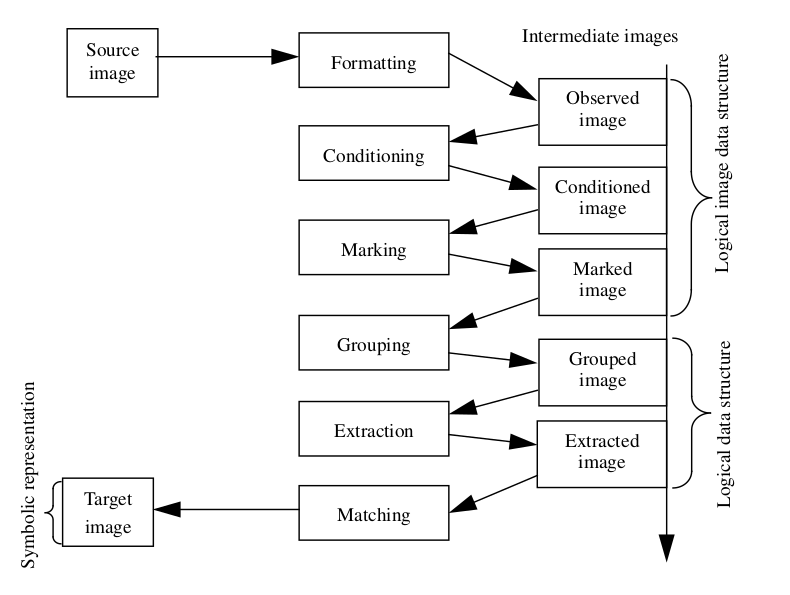
\includegraphics[width=0.8\textwidth]{image-recognition-steps}
	\caption{Steps involved in image recognition.}{\label{fig:image-recognition-steps}}
\end{figure}
%-------------------FIGURE END---------------------------

\paragraph*{The Image-Recognition Procedure/Steps}

The formatting step shoots an image by use of a camera and transforms the image into digital form (i.\ e.\ , pixels). The conditioning, marking, grouping,
extraction, and matching steps form a canonical division of the image recognition problem, where each step prepares and transforms the data required for the next step.
Depending on the application, it may be necessary to apply this sequence to more than one level of recognition and description. These five steps are:

\begin{steps}
\item \textit{Formatting}: The formatting step shoots an image by use of a camera and transforms the image into digital form (i.\ e.\ , pixels).
\item \textit{Conditioning}: 
		\begin{itemize}
			\item Conditioning is based on a model that assumes an image that can be observed is composed of information patterns, which are disturbed by irrelevant variations. \item Conditioning estimates the information pattern based on the observed image, so that noise can be suppressed. 
			\item Also, conditioning can normalize the background by ignoring irrelevant systematic or patterned variations. 
		\end{itemize}
		
\item \textit{Marking/Labeling}: 
		\begin{itemize}
			\item Marking is based on a model that assumes that information patterns have a structure in the form of spatial object arrangements, where each object is a set of interconnected pixels. 
			\item Marking determines to which spatial objects each pixel belongs.
		\end{itemize}
\item \textit{Grouping}: 
		\begin{itemize}
			\item The grouping operation identifies objects marked in the previous step by grouping pixels that are part of the same object.
			\item The grouping step includes the edge connection step. 
			\item A grouping operation that groups edges into lines is also called \textit{line fitting}.
			\item The grouping operation changes the logical data structure. 
			\item The original images, the conditioned, and marked images are all available as digital image data structures. 
		\end{itemize}
\item \textit{Extraction}: 	
			\begin{itemize}
				\item The grouping operation defines a new set of units, but they are incomplete because they have an identity but no semantic meaning. 
				\item The extraction operation calculates a list of properties for each pixel group. 
				\item Such properties can include center (gravity), surface, orientation, spatial moments, spatial grayscale moments, and circles.
			\end{itemize}
		
\item \textit{Matching}:
		\begin{itemize}
			\item When the extraction operation is finished, the objects occurring in an image are identified and measured, but they have no content meaning. 
			\item We obtain a content meaning by attempting an observation-specific organization in such a way that a unique set of spatial objects in the segmented image results in a unique image instance of a known object. 
			\item The matching operation determines how to interpret a set of related image objects, to which a given object of the three-dimensional world or a two-dimensional form is assigned.
			\item The classical method is template matching, which compares a pattern against stored models (templates) with known patterns and selects the best match.
		\end{itemize}
\end{steps}


\subsection{Image Synthesis}
Image synthesis is the process of creating new images from some form of image description. The kinds of images that are typically synthesized include:

\begin{itemize}
	\item \textit{Test Patterns}, Scenes with simple two-dimensional geometric shapes.
	\item \textit{Image Noise}, Images containing random pixel values, usually generated from specific parameterized distributions.
	\item \textit{Computer Graphics}, Scenes or images based on geometric shape descriptions. Often the models are three-dimensional, but may also be two-dimensional.
\end{itemize}
	Synthetic images are often used to verify the correctness of operators by applying them to known images. They are also often used for teaching purposes, as the operator output on such images is generally `clean', whereas noise and uncontrollable pixel distributions in real images make it harder to demonstrate unambiguous results. The images could be binary, gray level or color.

Image synthesis is an integral part of all computer-supported user interfaces and a necessary process to visualize 2D, 3D, or higher-dimensional objects. A large number
of disciplines, including education, science, medicine, construction, advertising, and the entertainment industry, rely heavily on graphical applications, for example:

\begin{itemize}
	\item \textbf{User interfaces}
	Applications based on the Microsoft Windows operating system have user interfaces to run several activities simultaneously and offer point-and-click options to select menu items, icons, and objects on the screen.
	
	\item \textbf{Office automation and electronic publishing}
	The use of graphics in the production and distribution of information has increased dramatically since desktop publishing was introduced on personal computers. Both office automation and electronic publishing applications can produce printed and electronic documents containing text, tables, graphs, and other types of drawn or scanned graphic elements. 
	
	\item \textbf{Simulation and animation for scientific visualization and entertainment}
	Animated movies and presentations of temporally varying behavior of real and simulated objects on computers have been used increasingly for scientific visualization. For example, they can be used to study mathematical models of phenomena, such as flow behavior of liquids, relativity theory, or nuclear and chemical reactions. Cartoon actors are increasingly modeled as three-dimensional computer-assisted descriptions. 
\end{itemize}

%Interactive computer graphics are the most important tool in the image production process since the invention of photography and television. With these tools, we cannot
%only create images of real-world objects, but also abstract, synthetic objects, such as images of mathematical four-dimensional surfaces.
%
%\subsubsection*{Dynamic Vs Static Graphics}
%The use of graphics is not limited to static images. Images can also vary dynamically. For example, a user can control an animation by adjusting the speed or changing
%the visible part of a scene or a detail. This means that dynamics are an integral part of
%(dynamic) graphics. Most modern interactive graphics technologies include hardware
%and software allowing users to control and adapt the dynamics of a presentation:
%
%\begin{itemize}
%	\item \textbf{Movement dynamics} 
%	
%	Movement dynamics means that objects can be moved or
%	activated relative to a static observer’s viewpoint. Objects may also be static while
%	their environment moves. A typical example is a flight simulator containing components that support a cockpit and an indicator panel. The computer controls the
%	movement of the platform, the orientation of the aircraft, and the simulated environment of both stationary and moving objects through which the pilot navigates.
%	
%	\item Adaptation dynamics: Adaptation dynamics means the current change of form,
%	color, or other properties of observed objects. For example, a system could represent the structural deformation of an aircraft in the air as a response to many different control mechanisms manipulated by the user. The more subtle and uniform
%	the change, the more realistic and meaningful is the result. Dynamic interactive
%	graphics offer a wide range of user-controllable modes. At the same time, these
%	modes encode and convey information, for example, 2D or 3D forms of objects in
%	an image, their gray levels or colors, and the temporal changes of their properties.
%\end{itemize}

\subsection{Image Transmission}
Image transmission takes into account transmission of digital images through computer networks. There are several requirements on the networks when images are transmitted:
\begin{itemize}
	\item The network must accommodate bursty data transport because image transmission is bursty (the burst is caused by the large size of the image).
	\item Image transmission requires reliable transport.
	\item Time-dependence is not a dominant characteristic of the image in contrast to audio/video transmission.
\end{itemize}

Image size depends on the image representation format used for transmission. There are several possibilities:

\subsubsection*{Raw image data transmission}
\begin{itemize}
	\item In this case, image is generated through a video digitizer and transmitted in its digital format. 
	\item The size can be computed in the following manner:
	\[
	Size = spatial\_resolution \times pixel\_resolution
	\]
	\item For example, the transmission of an image with a resolution of $ 640 \times 480 $ pixels and pixel quantization of 8 bits per pixel requires transmission of $ 3, 07,200 bytes $ through the network.
\end{itemize}

\subsubsection*{Compressed image data transmission}
\begin{itemize}
	\item In this case, the image is generated through a video digitizer and compressed before transmission. 
	\item Methods such as JPEG or MPEG are used to downsize the image. 
	\item The reduction of image size depends on the compression method and compression rate.
\end{itemize}

\subsubsection*{Symbolic image data transmission}
\begin{itemize}
	\item In this case, the image is represented through symbolic data representation as image primitives (e.g. 2D or 3D geometric representation), attributes and other control information. 
	\item This image method is used in computer graphics.
	\item Image size is equal to the structure size, which carries the transmitted symbolic information of the image.
\end{itemize}

\newpage\thispagestyle{empty}